\documentclass{amsart}
\usepackage{amssymb}
\renewcommand{\baselinestretch}{1.5}
\addtolength{\textwidth}{.2in}
\addtolength{\topmargin}{-.5in}
\addtolength{\textheight}{1in}

\usepackage{ifthen}
\usepackage{graphicx}
\usepackage{xcolor}

\newcommand{\versionNum}{$3.2$\ }

\newboolean{InTextBook}
\setboolean{InTextBook}{false}
\newboolean{InWorkBook}
\setboolean{InWorkBook}{false}
\newboolean{InHints}
\setboolean{InHints}{false}

%When this boolean is true (beginning in Section 5.1) we will use the convention
% that $0 \in \Naturals$.  If it is false we will continue to count $1$ as the smallest
%natural number (thus making Giuseppe Peano spin in his grave...)
 
\newboolean{ZeroInNaturals}

%This boolean is used to distinguish the version where we use $\sim$ rather than $\lnot$

\newboolean{LNotIsSim}

%The values of the last two booleans are set in ``switches.tex''

\setboolean{ZeroInNaturals}{true}
\setboolean{LNotIsSim}{false}


\let\savedlnot\lnot
\ifthenelse{\boolean{LNotIsSim}}{\renewcommand{\lnot}{\sim} }{}

%This command puts different amounts of space depending on whether we are
% in the text, the workbook or the hints & solutions manual. 
\newcommand{\twsvspace}[3]{%
 \ifthenelse{\boolean{InTextBook} }{\vspace{#1}}{%
  \ifthenelse{\boolean{InWorkBook} }{\vspace{#2}}{%
   \ifthenelse{\boolean{InHints} }{\vspace{#3}}{} %
   }%
  }%
 }


\newcommand{\wbvfill}{\ifthenelse{\boolean{InWorkBook}}{\vfill}{}}
\newcommand{\wbitemsep}{\ifthenelse{\boolean{InWorkBook} }{\rule[-24pt]{0pt}{60pt}}{}}
\newcommand{\textbookpagebreak}{\ifthenelse{\boolean{InTextBook}}{\newpage}{}}
\newcommand{\workbookpagebreak}{\ifthenelse{\boolean{InWorkBook}}{\newpage}{}}
\newcommand{\hintspagebreak}{\ifthenelse{\boolean{InHints}}{\newpage}{}}

\newcommand{\hint}[1]{\ifthenelse{\boolean{InHints}}{ {\par \hspace{12pt} \color[rgb]{0,0,1} #1 } }{}}
\newcommand{\inlinehint}[1]{\ifthenelse{\boolean{InHints}}{ { \color[rgb]{0,0,1} #1 } }{}}

\newlength{\cwidth}
\newcommand{\cents}{\settowidth{\cwidth}{c}%
\divide\cwidth by2
\advance\cwidth by-.1pt
c\kern-\cwidth
\vrule width .1pt depth.2ex height1.2ex
\kern\cwidth}

\newcommand{\sageprompt}{ {\tt sage$>$} }
\newcommand{\tab}{\rule{20pt}{0pt}}
\newcommand{\blnk}{\rule{1.5pt}{0pt}\rule{.4pt}{1.2pt}\rule{9pt}{.4pt}\rule{.4pt}{1.2pt}\rule{1.5pt}{0pt}}
\newcommand{\suchthat}{\; \rule[-3pt]{.5pt}{13pt} \;}
\newcommand{\divides}{\!\mid\!}
\newcommand{\tdiv}{\; \mbox{div} \;}
\newcommand{\restrict}[2]{#1 \,\rule[-4pt]{.25pt}{14pt}_{\,#2}}
\newcommand{\lcm}[2]{\mbox{lcm} (#1, #2)}
\renewcommand{\gcd}[2]{\mbox{gcd} (#1, #2)}
\newcommand{\Naturals}{{\mathbb N}}
\newcommand{\Integers}{{\mathbb Z}}
\newcommand{\Znoneg}{{\mathbb Z}^{\mbox{\tiny noneg}}}
\ifthenelse{\boolean{ZeroInNaturals}}{%
  \newcommand{\Zplus}{{\mathbb Z}^+} }{%
  \newcommand{\Zplus}{{\mathbb N}} }
\newcommand{\Enoneg}{{\mathbb E}^{\mbox{\tiny noneg}}}
\newcommand{\Qnoneg}{{\mathbb Q}^{\mbox{\tiny noneg}}}
\newcommand{\Rnoneg}{{\mathbb R}^{\mbox{\tiny noneg}}}
\newcommand{\Rationals}{{\mathbb Q}}
\newcommand{\Reals}{{\mathbb R}}
\newcommand{\Complexes}{{\mathbb C}}
%\newcommand{\F2}{{\mathbb F}_{2}}
\newcommand{\relQ}{\mbox{\textsf Q}}
\newcommand{\relR}{\mbox{\textsf R}}
\newcommand{\nrelR}{\mbox{\raisebox{1pt}{$\not$}\rule{1pt}{0pt}{\textsf R}}}
\newcommand{\relS}{\mbox{\textsf S}}
\newcommand{\relA}{\mbox{\textsf A}}
\newcommand{\Dom}[1]{\mbox{Dom}(#1)}
\newcommand{\Cod}[1]{\mbox{Cod}(#1)}
\newcommand{\Rng}[1]{\mbox{Rng}(#1)}

\DeclareMathOperator\caret{\raisebox{1ex}{$\scriptstyle\wedge$}}

\newtheorem*{defi}{Definition}
\newtheorem*{exer}{Exercise}
\newtheorem{thm}{Theorem}[section]
\newtheorem*{thm*}{Theorem}
\newtheorem{lem}[thm]{Lemma}
\newtheorem*{lem*}{Lemma}
\newtheorem{cor}{Corollary}
\newtheorem{conj}{Conjecture}

\renewenvironment{proof}%
{\begin{quote} \emph{Proof:} }%
{\rule{0pt}{0pt} \newline \rule{0pt}{15pt} \hfill Q.E.D. \end{quote}}


\addtolength{\abovedisplayskip}{0pt}
\addtolength{\belowdisplayskip}{24pt}
\addtolength{\abovedisplayshortskip}{0pt}
\addtolength{\belowdisplayshortskip}{48pt}


\begin{document}
\thispagestyle{empty}

\centerline{\Large Activity 23 -- Introduction to Proof}
\centerline{\large Venn diagrams}

\bigskip
\Large


\begin{enumerate}

\item Use the double inclusion strategy to prove that $A \setminus (B \cap C) \; = \;
A \setminus B \, \cup \,  A \setminus C$

\vfill

\newpage

\item Let $A = \{1, 2, 3, 4, 5, 6, 7\}$ and $B = \{2, 4, 6, 8, 10\}$. Write these
element in the appropriate regions in a Venn diagram for two sets.
\medskip

\input{2set_Venn.tex}
\medskip

\item On the 3-set Venn diagrams below shade the regions that corre-
spond to $A \cap (B \cup C)$ on the left and $(A \cap B) \cup (A \cap C)$ on the right.
\medskip

\centerline{
\begin{tabular}{ccc}
\input{3set_Venn-sm.tex} & \hspace{.25in} & \input{3set_Venn-sm.tex} \\
\end{tabular}
}

\newpage

\item Determine set-theoretic expressions for the shaded regions in the
Venn diagrams below.
\medskip

\centerline{
\begin{tabular}{ccc}
\input{3set_Venn-A.tex} & \hspace{.25in} & \input{3set_Venn-B.tex} \\
\end{tabular}
}

\vfill

\item Use rectilinear Jordan curves (simple closed curves made up of
horizontal and vertical line segments) to create a Venn diagram for
4 sets in general position.

\vfill

\vfill

\newpage

\item We can visualize the modus ponens argument form by placing
Socrates in the appropriate region and imposing the “All men are
mortal” condition by indicating a region on the diagram that must
be empty. Do it.

\vspace{.2in}

\input{2set_Venn-modus_ponens.tex}
\medskip

\newpage

\item In a similar fashion, create a visualization for the modus tollens
argument form:

\vspace{.2in}

\begin{tabular}{c}
All men are mortal \\
Zeus is not mortal \\ \hline
$\therefore$ Zeus is not a man
\end{tabular}

\vspace{.2in}


\input{2set_Venn-modus_ponens.tex}
\medskip

\newpage

\item Construct a Venn diagram for 4 sets using rectangles. (This is
slightly tougher than problem 5.)

\vfill



\item Use a Venn diagram for 4 sets to convince yourself of the validity
of the following containment statement

\[
(A \cap B) \, \cup \, (C \cap D) \; \subseteq \; (A \cup C) \, \cap \, (B \cup D).
\]

\vfill

\newpage

\item Use a Venn diagram to show that the following proposed set iden-
tity is false.

\[
\overline{A} \cap (B \cup C) = (B \cup C) \setminus (A \cap C)
\]

How could we use the intuition we developed from the Venn
diagram to construct a legitimate disproof? 
\medskip

\centerline{\begin{picture}(0,0)%
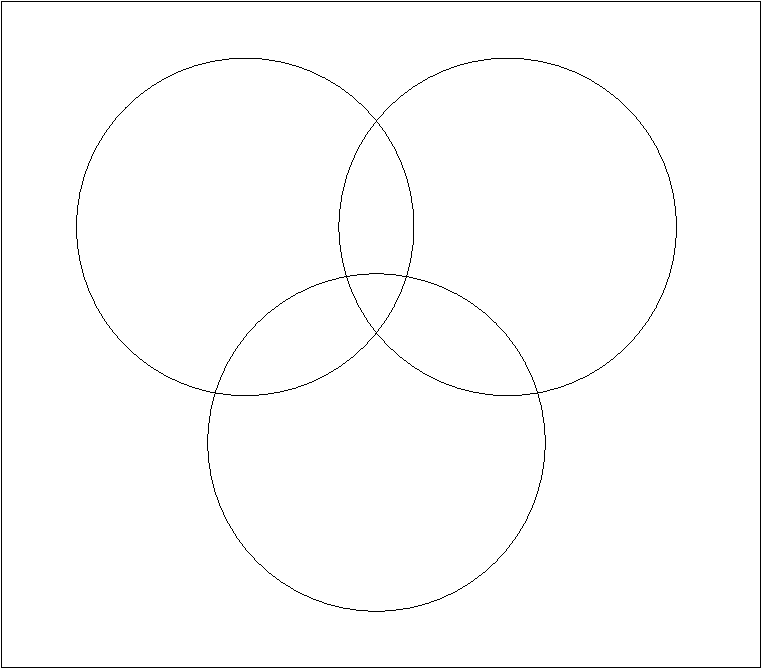
\includegraphics{./3set_Venn.pdf}%
\end{picture}%
\setlength{\unitlength}{3947sp}%
%
\begingroup\makeatletter\ifx\SetFigFont\undefined%
\gdef\SetFigFont#1#2#3#4#5{%
  \reset@font\fontsize{#1}{#2pt}%
  \fontfamily{#3}\fontseries{#4}\fontshape{#5}%
  \selectfont}%
\fi\endgroup%
\begin{picture}(6099,5349)(1189,-5398)
\put(2326,-1036){\makebox(0,0)[lb]{\smash{{\SetFigFont{12}{14.4}{\familydefault}{\mddefault}{\updefault}{\color[rgb]{0,0,0}A}%
}}}}
\put(6001,-1036){\makebox(0,0)[lb]{\smash{{\SetFigFont{12}{14.4}{\familydefault}{\mddefault}{\updefault}{\color[rgb]{0,0,0}B}%
}}}}
\put(1276,-286){\makebox(0,0)[lb]{\smash{{\SetFigFont{12}{14.4}{\familydefault}{\mddefault}{\updefault}{\color[rgb]{0,0,0}U}%
}}}}
\put(4126,-4861){\makebox(0,0)[lb]{\smash{{\SetFigFont{12}{14.4}{\familydefault}{\mddefault}{\updefault}{\color[rgb]{0,0,0}C}%
}}}}
\end{picture}%
}

\newpage

\item Illustrate the absorption laws for sets on Venn diagrams.


\end{enumerate}


\end{document}
